\section{Vorgehen}

Die Vorgehensweise orientiert sich an Scrum, wird jedoch angepasst auf dieses Projekt.
Scrum ist aine agile Projektmethode, die oft in Softwareentwicklung verwendet wird. Dabei wird in Zeitboxen, die Sprint genannt werden, gearbeitet. Pro Sprint gibt es mehrere Tasks, die bearbeitet werden sollen, sowie Sprintziele. Dies wird in diesem Projekt so gemacht.

Normalerweise gibt es taegliche Synchronisationsmeetings. Hier werden diese woechentlich durchgefuehrt, ansonsten wird eher asynchron gearbeitet.

Sprintreviews werden durchgefuehrt im Rahmen der Besprechung der Testatabgaben mit dem Coach. Retrospektiven werden nicht strukturiert durchgefuehrt, jedoch wi

\subsection{Projektorganisation}

Da es sich um eine interdisziplinarische Produktentwicklung handelt, wurde das Team aus jeweils zwei Studierenden aus den Studiengängen \acrfull{elektrotechnik}, \acrfull{informatik} und \acrfull{maschinentechnik} zusammengeführt. In Abbildung \ref{fig:Organigramm} ist die Projektorganisation ersichtlich. 

Im Team wurde Alina Meyer als Projektleiterin gewählt. zudem benötigt es für die Mechanische und Elektrische Werkstetten in der Hochschule Luzern jeweils einen zuständige Person im Team. Welche dem Ivan Zimmerman (\acrshort{elektrotechnik}) und Elias von Atzigen (\acrshort{maschinentechnik}) zugeteilt wurde.

Die klare Aufteilung der Rollen ermöglicht es dem Team, effizient und zielgerichtet an der Entwicklung des Projekts zu arbeiten. Durch diese Struktur wird gewährleistet, dass jede technische Disziplin angemessen abgedeckt ist und die Kommunikation innerhalb des Teams reibungslos funktioniert.

\begin{figure}[h]
\centering
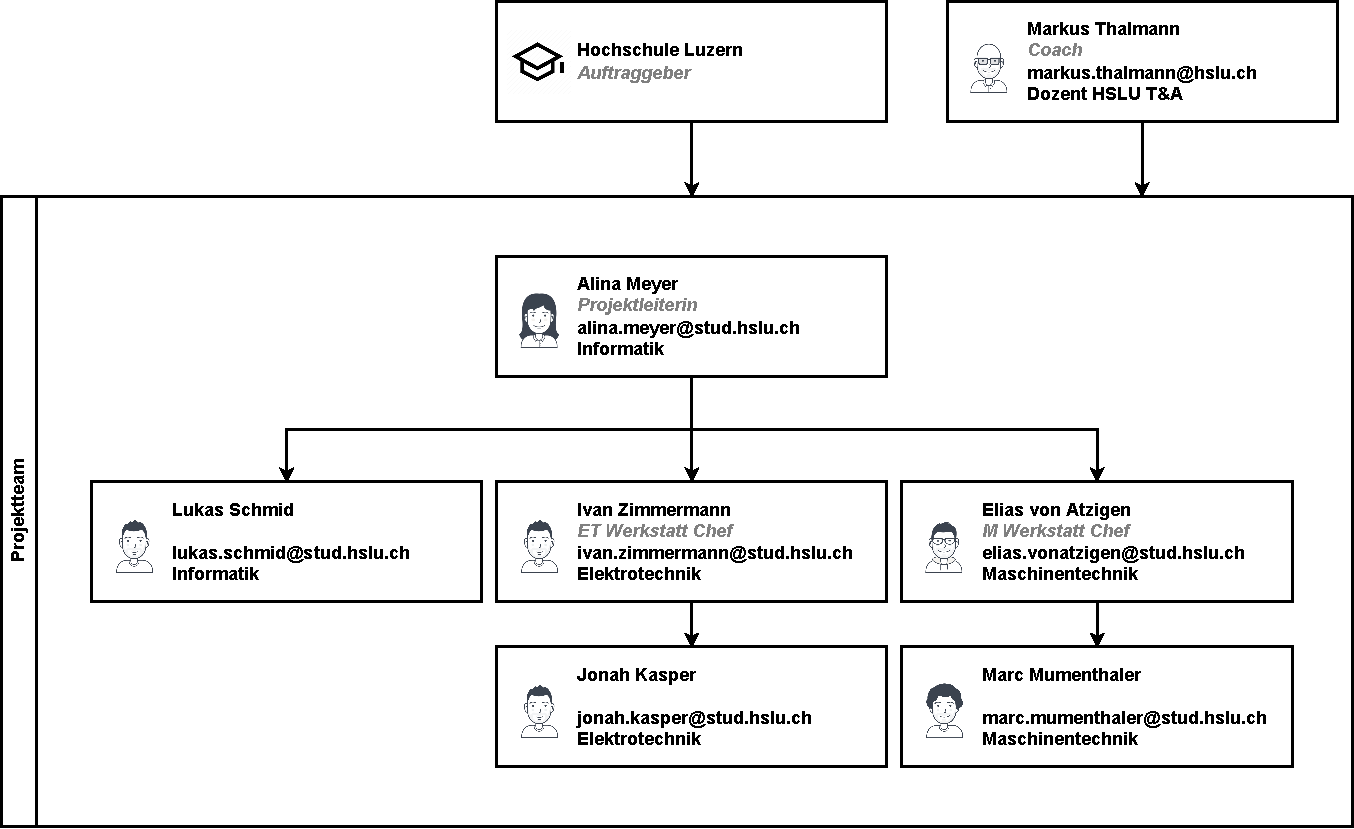
\includegraphics[width=\textwidth]{img/Projektorganisation.pdf}
\caption{Organigramm}
\label{fig:Organigramm}
\end{figure}

\subsection{Datenaustausch}


\subsection{Design Thinking}